\documentclass{article}
\usepackage[T1]{fontenc}
\usepackage{lmodern}
\usepackage{graphicx}
\usepackage{amsmath,amssymb}
\usepackage[a4paper,margin=2cm]{geometry}
\usepackage[absolute,overlay]{textpos}
\setlength{\TPHorizModule}{1mm}
\setlength{\TPVertModule}{1mm}
\usepackage[indonesian]{babel}
\usepackage{hyperref}
\setlength{\emergencystretch}{2em}
% unit: Halaman 28

\begin{document}

% === Halaman 28 (python/native) ===

Satu putaran di dalam jaringan Feistel secara lengkap:

1

2

3

4

5

6

7

8

11

12

13

14

15

16

17

18

9

10

21

22

23

24

25

26

27

28

19

20

31

32

29

30

1

2

3

4

5

6

7

8

11

12

13

14

15

16

17

18

9

10

21

22

23

24

25

26

27

28

19

20

31

32

29

30

28

29

24

25

21

20

16

17

13

12

4

5

8

9

32

1

1

2

3

4

5

6

7

8

11

12

13

14

15

16

17

18

9

10

21

22

23

24

25

26

27

28

19

20

31

32

29

30

33

34

35

36

37

38

41

42

43

44

45

46

47

48

39

40

1

2

3

4

5

6

7

8

11

12

13

14

15

16

17

18

9

10

21

22

23

24

25

26

27

28

19

20

31

32

29

30

33

34

35

36

37

38

41

42

43

44

45

46

47

48

39

40

S4

control

input symbol

output symbol

1

2

3

4

5

6

7

8

11

12

13

14

15

16

17

18

9

10

21

22

23

24

25

26

27

28

19

20

31

32

29

30

S3

control

input symbol

output symbol

input symbol

S5

control

input symbol

output symbol

input symbol

S6

control

input symbol

output symbol

input symbol

S7

control

input symbol

output symbol

input symbol

S8

control

input symbol

output symbol

input symbol

S1

control

input symbol

output symbol

input symbol

S2

control

input symbol

output symbol

input symbol

1

2

3

4

5

6

7

8

11

12

13

14

15

16

17

18

9

10

21

22

23

24

25

26

27

28

19

20

31

32

29

30

Right Half i-1

Round Key i

1

2

3

4

5

6

7

8

11

12

13

14

15

16

17

18

9

10

21

22

23

24

25

26

27

28

19

20

31

32

29

30

1

2

3

4

5

6

7

8

11

12

13

14

15

16

17

18

9

10

21

22

23

24

25

26

27

28

19

20

31

32

29

30

1

2

3

4

5

6

7

8

11

12

13

14

15

16

17

18

9

10

21

22

23

24

25

26

27

28

19

20

31

32

29

30

O+

O+

Left Half i-1

Right Half i

Sumber: Cryptography and Network Security

Chapter 3, Lecture slides by Lawrie Brown

Modified by Richard Newman

Ri-1

32 bit

E(Ri-1)

Ekspansi menjadi 48 bit

48 bit



Ki

48 bit

A

K

R

E

i

i

=



−)

(

1

S1

S8

...

B

Matriks substitusi

32 bit

48 bit

P(B)

32 bit

f

28

% deskripsi: gambar native xref 109
\noindent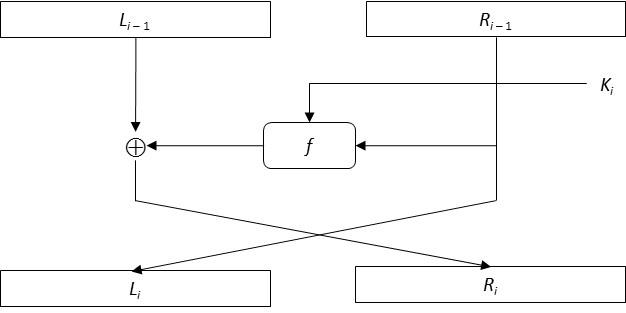
\includegraphics[width=0.85\textwidth]{../../images/python/page_028_img_01.jpeg}

\end{document}
